\section{Background}

% % Brief "what is this?" section to explain structure of background
% If we are to visualize accessibility,
% a general understanding of research in both accessibility and cartography is necessary.
% After briefly presenting both fields,
% I will relate the two together
% providing a more focused synthesis of the aspects most relevant to this thesis.

% \begin{itemize}
% 	\item Define terms more in depth (cartography, map, accessibility...)
% 	\item Small history recap of the relevant advances in the field of cartography
% 	\item Cartographic interaction theory
% 	\item Web mapping advances and technologies
% 	\item Interactive accessibility presentations and other relevant maps: go over some previous implementations and solutions.
% \end{itemize}

% Cartography - How we got to where we are now, what this means for the topic
\subsection{Maps, cartography and cartographic interaction}

\subsubsection{Defining \enquote{map}}
While the meaning of the word \textit{map} seems obvious,
defining it has been anything but simple for cartographers.
In a review of various historical writings \textcite{and1996}
found 321 unique definitions for the word.
Most of these definitions shared the premise that
maps are representations of the surface of the earth,
but, other than that, not many similarities were found.
More recent efforts in defining the word range
from lengthy attempts at precise delineation
(for example \textcite{ica2003})
to much shorter definitions (for example \textcite{kra2017}).
Currently, the \acrlong{ica} (\acrshort{ica}),
the authoritative international body for cartography,
defines map as \enquote{an abstract visual representation of the geo-environment}
\parencite{ica2019}.

% What map for real?
Even though quite concise,
\acrshort{ica}'s definition has received its fair share of critique as well.
For example, \textcite{lap2021} note that
a map can be a concrete object or have concrete qualities
instead of being strictly abstract,
and be perceived with senses other than vision.
The word \enquote{geo-environment} is problematic too.
It would limit maps to depicting only earth
-- an issue found in many map definitions \parencite{tyn2014} --
as well as introduce possible confusion with themes such as
environmental sustainability \parencite{lap2021}.
As a response, \textcite{lap2021} suggest that,
instead of a given environment or a type of map,
\textit{spatial relationships} should be the starting point of defining what a map is.
Thus, \citeauthor{lap2021} arrive at the following definition:
\enquote{a map is a generalized representation of spatial relationships}.
A few years earlier, \textcite{tyn2014} shared much of the same sentiments,
defining a map as \enquote{a graphic representation that shows spatial relationships}.
While in her definition \citeauthor{tyn2014} specifies maps as something graphic,
both authors are in agreement that maps are representations,
and that representing spatial relationships is what makes a representation a map.

% What does "representation" mean?
% \textcite{mac2004}, along the same lines, goes as far as to say

\subsubsection{Cartography as a science}
% What cartography?
% This paragraph could move to the definition section above
It is known that
maps have been made and used in human communities for thousands of years
(for example \textcite{hsu1993, sch2014}).
However, cartography,
not as in the practice of mapmaking but as in an established science,
is much younger.
In fact, \textcite{woo2003, kai2020, cra2018} argue that
the discipline of cartography dates back only to the early 1900s,
since that is when a scientific body of theory on maps started to form.
Before that, it was mainly the mathematical theory on map projections
and the production of topographical maps
that were associated with cartography \parencite{kai2020}.
In the time that cartography has been considered its own science,
change has been a constant in the discourse within the discipline \parencite{mac2004} --
% the discipline has reinvented itself many times.
cartography is as dynamic as the topics that people map,
or the methods they use to map said topics \parencite{tyn1992, tyn2014}.
Consequently,
the term cartography has been difficult to define \parencite{kry1995},
and even if a definition is agreed upon,
it should be considered a product of the time period
in which it was envisioned \parencite{tyn1992, and1996}.
Currently, \acrshort{ica} defines cartography as
\enquote{the science, art, and technology of making and using maps}.
\parencite{ica2019}.

To better understand the discipline of cartography,
it is essential to acknowledge
the field's multidisciplinary, dynamic and multi-paradigmatic nature.
Often, methods of other disciplines are used in cartography,
and, perhaps even more often,
maps and cartography act as tools for other disciplines \parencite{kai2020}.
What these overlapping disciplines are, changes as the field evolves
and the paradigms within cartography shift
\parencite{kai2020, mac2004}.
% TODO list relevant fields -> tell that their relevance changes through paradigm shifts
% Maps and cartography are tools for all spatial sciences
% Mathematics
% Computer science
% Psychology
% Social sciences
At first, as stated earlier,
it was mathematics that was the science most relevant to mapmaking and cartography.
Representing the curved surface of earth  %, a geoid in shape,
on a surface of a different shape, often a plane when maps are concerned,
requires a mathematical transformation \parencite{tyn1992}.
In the context of cartography, this transformation is called a map projection.
The effects the projection has on a map vary by
the properties of the specific transformation used and the scale of the map,
but are always present as distortions introduced to the map \parencite{tyn1992}.
This has direct influence on how a map works, both in the sense of
its visual composition and
how the map reader understands the map \parencite{ker2018}.

% For example producing general purpose maps using a projection intended for navigation purposes.

% 1950
A map only gains meaning when it is read \parencite{gri2017}.
The process of reading a map comprises, for example,
perceiving, judging and reasoning,
often problem-solving and learning too \parencite{mon2002}.
All these are cognitive processes \parencite{apacog},
so it is clear how the field of psychology is fundamentally tied with cartography.
Initially, the link between cartography and psychology
was motivated by a shift in the discourse within cartography:
Like many disciplines post World War II,
cartography strived for credibility through empirical science.
Instead of objects of art and graphic design,
maps should be considered scientifically dissectable representations
with the primary function of conveying information \parencite{rob1952}.
Called functional map design,
this movement in cartography employed scientific methods,
especially those of psychology,
to find objectively provable rules
for producing as functional as possible maps \parencite{mon2002}.
For example,
research to optimize cartographic methods, such as symbology or labelling,
was carried out by utilizing empirical studies on human perception \parencite{mac2004}.

% ken2018, Boa2017, fai2021
In addition to studying and improving the function of maps,
functional map design had an essential role in conceptualizing \textit{how} maps function.
Already present in the work of \textcite{rob1952},
the initial concept of map function was strongly linked to graphical communication.
Drawing inspiration from studies in psychology and information sciences,
this discourse was only strengthened in the following decades
in what can be referred to as the paradigm of cartographic communication \parencite{fai2021}.
The premise of cartographic communication is
that a map is a component in a communication system,
in which its purpose is to transport knowledge to the map reader
\parencite{Boa2017}.
Many varyingly intricate models of cartographic communication exist,
but the main principles are that \parencite{ken2018}:
\begin{enumerate}
	\item The knowledge a map reader gains from reading a map is that of the mapper's,
	just transferred through cartographic communication.
	\item The main purpose of the cartographic method is
	to minimize the loss of information in that transfer.
\end{enumerate}

% With the latter half of the twentieth century,
% the relevance of computer science
While the concept of cartographic communication was
a widely used premise in cartographic inquiry \parencite{ken2018},
the discipline soon evolved into other directions.
The latter half of the twentieth century saw many developments in computer science
that, in turn, enabled notable advances in cartography:
for example computer-stored spatial data,
computer-assisted spatial modelling, and, eventually,
maps presented as computer graphics \parencite{kai2020}.
As a result, the function of maps widened
and the paradigm of cartographic communication was found quite limiting.
For example, if the acts of making and reading maps were strictly equivalent to
encoding and decoding messages,
no new knowledge would be constructed by the map reader in reading a map \parencite{mac2004}.
As maps started to increasingly be used
as exploratory and analytical devices,
this was not necessarily the most fitting way of thinking of them.
Often the mapmaker and reader were the same person,
and the purpose of the map was not strictly to communicate
but also to facilitate analytical thinking
-- in other words produce new knowledge \parencite{tob2000, ant1999, kry1995}.
With its roots in analytical cartograpghy \parencite{tob1976},
this concept of map usage first gained significant traction known as
cartographic visualization \parencite{ant1999},
a subset of the wider trend of scientific visualization
enabled by computer graphics \parencite{nie1997}.
Currently, this paradigm is best known in the form of geovisual analytics
which is also considered a science in its own right \parencite{rob2017b}.

\enquote{The map is never neutral} \parencite[p.~15]{har1989}.
\citeauthor{har1989}'s view on the nature of maps set in motion
a notable shift in the cartographic discourse
that became known as critical cartography \parencite{cra2018}.
At the core of critical cartography is the notion that
maps can never be objective sources of truth --
rather, they are socially constructed instruments of power
that ultimately reflect the ideologies of their makers \parencite{har1989}.
This sociocultural critique of maps and mapmaking
heavily contrasted the earlier paradigms in cartography.
Previously, the often implicitly authoritative map was
assumed to be capable of neutral knowledge transfer,
and the methods by which it was studied were in many cases positivist in nature
\parencite{cra2018, fai2021}.

% Multi-paradigm present day
As one main takeaway it should be recognized that
while I presented the above paragraphs quite linearly,
the multiple paradigms and disciplines relevant to cartography co-exist.
For example,
the role of mathematics is always essential to cartography --
be it the study of map projections \parencite{ker2018},
or the development of the mathematical methods
by which phenomena are represented on a map
\parencite{fra2000}.
Cartographic studies focusing on the empirical study of human perception
have continued and been applied to new types of maps (for example \textcite{col2009}),
and models of map communication still act as a basis for
much of cartographic research \parencite{ken2018}.
The paradigm of geovisual analytics is thriving,
largely enabled and amplified by the advances of geographic information systems (\acrshort{gis})
and other platforms that advance the analytical and explorative power of maps
\parencite{rot2013a, kra2017, lv2017}.
Critical cartography has lead to the acknowledgement of the power of maps
\parencite{cra2018, pic1995},
and to qualitative and mixed-methods approaches to studying and crafting them
\parencite{suc2000, cop2009}.

% Draws heavily from the paradigm of graphical communication,  % useless line?
% \textcite{bal1966} propose a term, "graphicacy",
% to relate the importance of graphical communication to literacy, articulacy and numeracy.
% Among the pioneers of this way of thinking about maps was \textcite{kol1969},
% who explicitly regarded maps as communication systems.

% Critique of positivism, parallel to psychophysics
% As the communication model evolved and eventually gained competition,


% Fields relevant in the sense of development of the tools of cartography,
% for example computer science \parencite{mon1985}


% \parencite{kai2020}


% % 1970
% % Cartography as graphic communication.
% The second was the change in how a map is thought to work.

% However, there have been numerous objections to the paradigm of Cartography as a form of communication.
% Firstly, there is the issue of communication versus function:
% A mapmaker might not have an intent to communicate any particular message to begin with.

% Also, implicit vs explicit:
% the message the map reader extracts from a map might differ from the one intended, or


% % Moving on from these
% Art and science \parencite{mac2004, tyn1992}  % compare these

% 1990
% - More interlinked with GIS
% - critical / qualitative GIS too

% 2010-the present -> interactive
% The change in cartography
% Rise of open source \textcite{pet2015}


% Different types of maps

% TODO
% For most of humanitys history maps have been a tool to describe the physical world,
% used for navigation and comprehending places etc
% Nowadays data visualization
% Presenting the world (locations) vs presenting data linked to locations (thematic mapping, \parencite{tyn1992})

\subsubsection{Cartographic interaction and interactive maps}

% What is interactive cartogra
So far I've referred to any persons viewing maps mostly as map readers.
Cartographic interaction refers to a process
in which the map reader interacts with the map,
thus becoming an active map user, even a mapmaker,
instead of a passive map reader \parencite{rot2017}.
The concept of interaction is rooted in social theory,
where it comprises the actions and reactions in
two-way communication between humans \parencite{ken1996}.
However, with the advance of computer technology,
interaction theories have been increasingly applied and developed
in the context of dialogue between humans and computers \parencite{qui2008}.
This is known as \acrlong{hci} (\acrshort{hci}).
In addition to the process, \acrshort{hci} is a field of research examining
the function of interactive user interfaces (\acrshort{ui})
and user experience (\acrshort{ux})
in enabling dialogue between computers and humans \parencite{car1997, hor2017}.
Interactivity, then, can be
a property, a perception, or an experience \parencite{lan2023},
and, depending on how it is conceptualized,
it can be modelled and studied in a multitude of ways \parencite{smu2009}.
Additionally, it must be noted that interaction and interactivity are factors
that depend not only on the technologies and
contexts of dialogue, but also on people’s perceptions and capabilities
\parencite{kio2002, duc2018}.

At the most general level of definition,
cartographic interaction can refer to
any type and level of interaction with any kind of map \parencite{pet1998}.
In fact, \citeauthor{pet1998} goes as far as to argue
that the static map of the modern times is the exception:
Interaction, for example mapmaking as a communicative aid in social contexts
(figure \ref{fig:paper interactive map}),
has been the norm of making and understanding maps
before they were transformed into static artefacts,
be it printed or digital images.
In this thesis I approach cartographic interaction as
two-way communication between a map and a map user,
but limit it to digital maps and \acrshort{hci}.
As defined by \textcite[p.~64]{rot2013b},
\enquote{cartographic interaction is the dialogue between a human and a map
mediated through a computing device}.
This is a relevant approach considering
that the mediums in which people interact with maps today
are predominantly and increasingly digital \parencite{mei2019}.
Digital environments also enable more ways to interact with maps
and to construct interactive map presentations \parencite{rot2013b, mei2019}.
Considering the aforementioned definition of cartographic interaction,
I deduce that, in the context of this study,
an interactive map is a digital one (figure \ref{fig:digital interactive map}),
and for it to be considered interactive it has to
enable manipulation by the map user.

\begin{figure}[H]
	\centering
	\includegraphics[width=0.7\textwidth]{visual/figures/photos/paper_interactive_map.png}
	\caption{
		An interactive paper map about how people experience travel in urban space.
		Constructed in a workshop setting,
		it enables cartographic interaction
		through manipulation by post-it-notes and annotations.
		Here the process of mapmaking is also a social one,
		as it both facilitates and is facilitated by
		human to human interaction about the mapped topics.
		Photo by Christoph Fink.
	}
	\label{fig:paper interactive map}
\end{figure}

\begin{figure}[H]
	\centering
	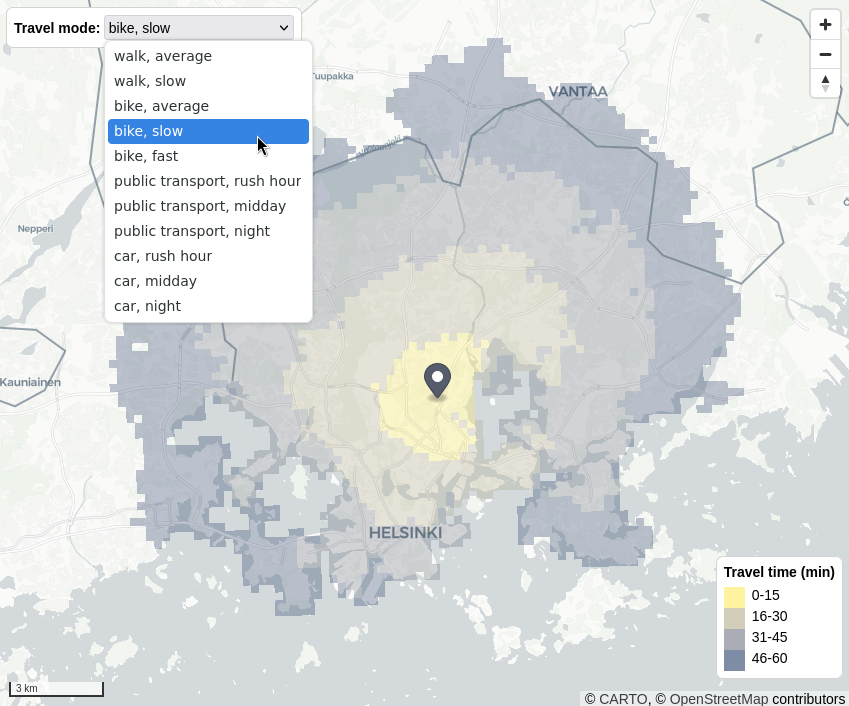
\includegraphics[width=0.8\textwidth]{visual/figures/screenshots/digital_interactive_map.png}
	\caption{
		A screenshot of a digital interactive map about travel times.
		In digital interactive maps
		cartographic interaction happens through a graphical UI,
		where the map can be manipulated by the user.
		In this example, the user can for example
		change the extent of the map by panning and zooming,
		and change the mapped data by selecting different options in a drop-down menu.
	}
	\label{fig:digital interactive map}
\end{figure}

In the previous definition of cartographic interaction there are three components:
the human as the user, the map as the interface,
and the computing device as the technology that enables the interaction.
% Arguably, there is a fourth component too: the dialogue.  % TODO
While cartographic interaction as a concept should be approached as
the sum of its parts \parencite{rot2013b},
studies on cartographic interaction can take on perspectives
that emphasize given subsets of these components.
For example, \textcite{col2009} approach the topic from a user-centric perspective,
\textcite{rot2013a} has an interface-centric focus in
taxonomizing various interaction primitives in map interfaces,
and \textcite{oym2021} develop a technological method and an implementation
for producing interactive maps.
I should also stress that I do not wish to imply that these studies
only recognize the singular components of cartographic interaction
I've associated with them here.
Rather, they approach the topic from a perspective relevant to their respective goals,
but they do account for the other components as well.

% HCI
The components of cartographic interaction widen the scope of cartography,
also further motivating and calling for
multidisciplinary approaches in the field \parencite{rot2013b}.
As maps become interfaces,
\acrshort{ui} and \acrshort{ux} research and design becomes
part of the process of mapmaking \parencite{rot2015}.
Thus, the research, theories and methods in \acrshort{hci}
and usability engineering (\acrshort{ue}) have been notable influences
digital interactivity has introduced to the discipline of cartography \parencite{rot2017}.
These can for example be new empirical approaches such as
data acquisition through system or application level recording and storage of
user interactions with map-based digital interfaces \parencite{oom2015}.
Research on the different technological aspects and modes of \acrshort{hci}
has also been carried out in cartographic contexts,
for example by evaluating different input devices and methods
used in interacting with web map applications \parencite{wu2011}.

% UE
The usability of interactive map presentations has been studied with
usability metrics often employed in \acrshort{ue} research more widely.
These include but are not limited to
user satisfaction (how content users are with an interface having used it),
efficiency (how quickly users complete tasks with an interface)
and effectiveness (how successful users are at completing tasks with an interface)
\parencite{col2009}.
When considering usability, it should also be noted that interactive maps,
often relying solely on computer graphics for all aspects of their interface,
introduce different accessibility requirements and challenges
especially for visually impaired users \parencite{duc2018}.
Still, it has been shown that interactive maps can satisfy these requirements,
potentially even better than static accessibility-oriented map designs:
By introducing methods such as tactile and audio interaction,
interactive maps have been observed to be more efficient and satisfactory interfaces
for visually impaired users when compared to tactile static maps \parencite{bro2015}.
In general, as informed by \acrshort{ue},
the need for user-inclusion in studies on cartographic interaction has been recognized,
and user-centred design practices are considered beneficial to map interface design
\parencite{niv2007, rot2017}.

Even though briefly mentioned earlier,
geovisual analytics should also be highlighted as
a discipline that is especially relevant to cartographic interaction.
Defined as \enquote{the science of analytical reasoning with
spatial information as facilitated by interactive visual interfaces}
\parencite{rob2017b},
it is clear that geovisual analytics is largely enabled by
cartographic interaction.
In contrast to research in \acrshort{hci} and \acrshort{ue} --
both fields that are focused mainly on interfaces as primary objects of study \parencite{rot2017} --
studies in geovisual analytics are more concerned with
how those interfaces enable and support analytical processes \parencite{rob2017b, and2010}.
An analytical process in this context refers to
exploring data and extracting insight from it,
assessing and contrasting different data and insights,
and presenting and reasoning about results \parencite{mac2017}.
From the perspective of cartography and especially interactive maps,
this type of approach includes the map interface in all stages of reasoning.  % includes? TODO
This inherently 
% tasks as examples

% what these tasks are -> what the map do -> interaction primitives
Continues with a short assessment of relevant fields,
contrasting them to ones applicable to cartography in general (the previous section): 
\acrshort{hci}, \acrlong{ue} (\acrshort{ue}), information visualization, visual analytics \parencite{rot2015}

% at the level of cartographical theory rot 2013b

% yi2007, rot2013a
Close this section with interactive maps in more detail:
Interaction primitives, different levels and types of interaction.
Different uses.





% Interactive
% In the following, the term “in-teractive” is used rather than “dynamic” to distinguish display updates evoked by the user(interaction) from display updates evoked by the system (such as animation, a form of car-tographic representation)phy - broadly  % FIXME copypasta


% \parencite{kra2017}
% The traditional ‘authoritative’ view of the map being a carefully crafted product
% by the cartographer, aimed at visually communicating a complete, mostly static database
% of known geographic facts to a user, has turned into a participatory and collaborative perspective.
% The map has moved beyond the static window to the world and become an
% interactive, mobile, dynamic and collaborative interface between a human, groups of
% people and the dynamically evolving environment



% The nature of interactive cartography
% More than a map: ui, ux
% What even is an interactive cartographer?
% A map is both the for of presentation, as well as the method of interaction
% -> a more complex map means basically a user interface -> need for UI library
% \textcite{rot2013a, rot2013b}

\subsection{Crafting interactive maps}
\subsubsection{Maps as digital applications}

Technological implications of map interaction,
technology being an enabling and a limiting factor in map interaction.

% The influence of technology on interactive maps and cartography.
% Also, the mapmaker is more often a software developer than a cartographer.
% How much of innovation is more of "this is cool",
% versus "this is a cartographically informed way to present something".

The platforms on which interactive maps are used:
Desktop software, mobile, web ...

\subsubsection{Web maps and mapping technologies}

Why web-based applications are the norm
(in general and, for much of the same reasons, in the context of maps).

Define web map

The relevant terms and software architechture (in web context):
At least the concepts of front / backend and server requests / responses
are pretty essential to understanding anything about the technical side.

The relevant technologies, the tools with which interactive maps are made:
web mapping and user interface libraries, backend solutions
(not every technology but a concise overview)

\subsection{Cartographic presentation of accessibility}

Different conceptualizations of accessibility,
their implications in presenting the phenomenon.

In general: people, transport, activities make up accessibility.
A multi-location, multimodal, multi-temporal phenomenon.

Approaches in visualizing accessibility:
Examples of static and interactive accessibility maps.
Simple measures vs complex measures,
High interactivity vs low interactivity.

Isochrones as an example of a simple measure / visualization approach:

\begin{figure}[H]
	\centering
	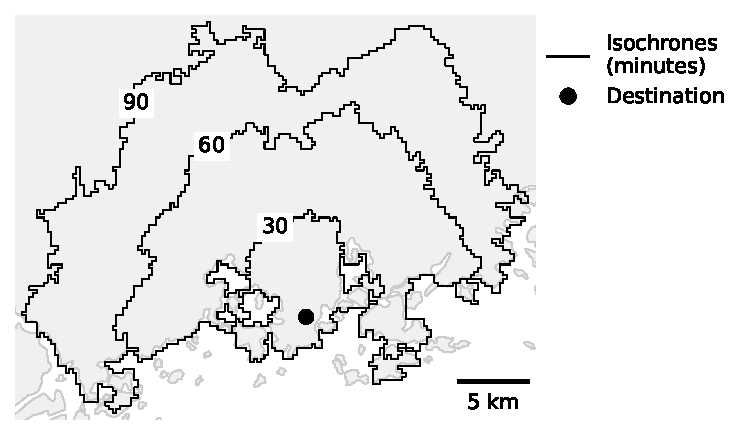
\includegraphics[width=0.6\textwidth]{visual/figures/ttm/isochrone_lines.pdf}
	\caption{Isochrones}
	\label{fig:isochrone lines}
\end{figure}

\begin{figure}[H]
	\centering
	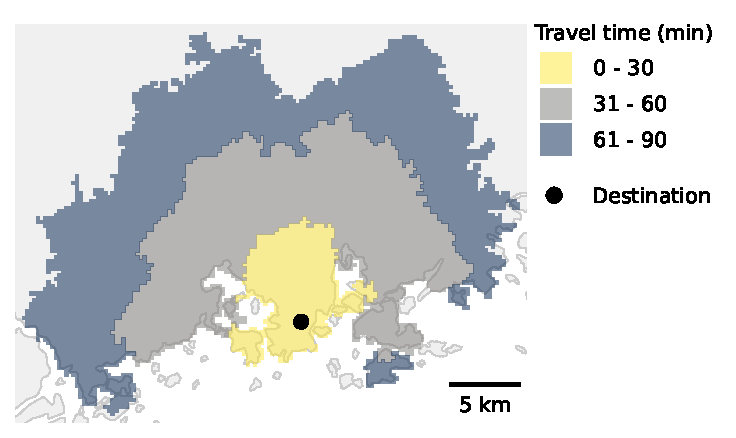
\includegraphics[width=0.6\textwidth]{visual/figures/ttm/isochrone_areas.pdf}
	\caption{Areas between isochrones}
	\label{fig:isochrone areas}
\end{figure}

SIDENOTE: How should I refer to isochrones when I mean the polygons instead of lines?

% TODO
% Mention tradeoffs (detail - speed) -> leads to methods
% Crafting any cartographic presentation is much about tradeoffs.
% Often these tradeoffs are concerned with the visual composition of the presentation --
% what the map can and should try to communicate.

% TODO
% Previous presentations can be very precise, but locked to a single place

